\section{Introduction}
\label{sec:intro}
%%AZ.8.29: Readability from here below needs work.
% % Caleb: describe this in the language of control bottlenecks
%%AZ.8.29: This is not necessarily true, it depends on the policy. You mean for a stochastic policy that either succeeds or fails with near equa probability.
%%AZ.8.29: below reads like AI.
%%AZ.8.29: can you be a bit more precise about how you do this?
% Caleb: I think this is too vague, because the SM is already a discounted occupancy, which is similar to a probability (and dominate the size). 
% Caleb: This might better be described by normalization still, and then just using "normalized mass", since at some level I think it isn't really a probability
% Caleb: If we use the language of normalization above, we can probably use more specific language here (normalizing the inner product spaces of classic successor measure algorithms)
%%AZ.8.29: L30 also reads like AI.
%%AZ.8.29: This jump to implementation details is too sudden. Need a better link between high-level intuition and actual implementation.

% Get to the point intro
The successor measure (SM) of a policy is its discounted distribution over future states, independent of any reward, so the value of a reward specified only after training is simply its expectation under the SM.
Reinforcement Learning  (RL) methods such as Forward-Backward (FB) representations use these predictions to learn policy families for zero-shot control~\citep{touati-neurips21a,touati-iclr23b,agarwal-icml25a}.
However, in practice even small errors in the approximation can lead these methods to give the wrong ranking to actions, which matters specifically for problems where this ranking is important for downstream control.
In manipulation, FB can reach the correct object yet fail to grasp it securely or place it at the goal~\citep{mohan-rlbrew26a}.
This raises a natural question: \emph{Why does FB fail to capture such precise behavior?}

% Bottlenecks
We hypothesize that this failure arises because of \emph{control bottlenecks}: transitions that are necessary passages to valuable regions where the choice of action substantially affects return.
For example, passing through a doorway determines which side of an environment can subsequently be explored; making the correct contact during an insertion determines whether the object can subsequently be manipulated; and establishing a stable grasp determines whether an object can be carried at all.
Although these decisions may occupy only a few steps, their consequences extend far into the future.
Methods that learn SM representations must preserve those consequences well enough to distinguish the actions that enable progress.


\begin{figure}[htb]
    \centering
    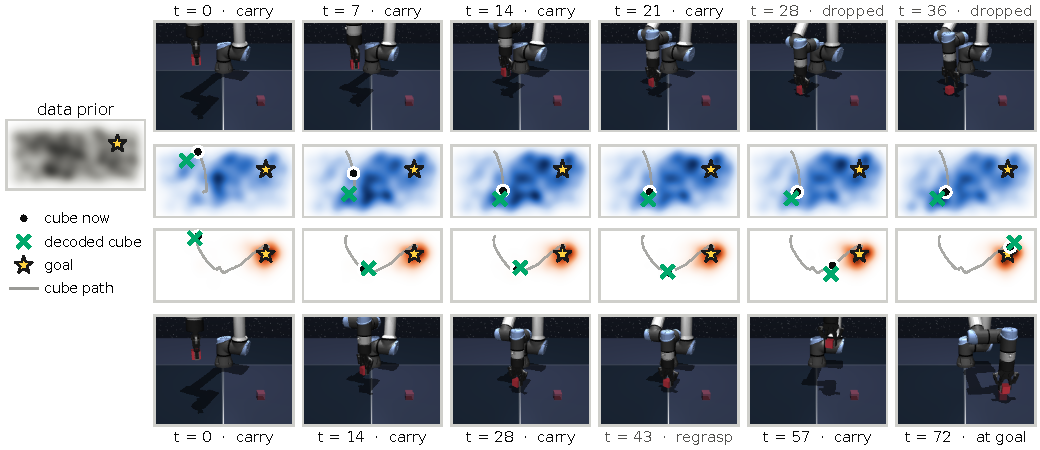
\includegraphics[width=\textwidth]{ICLR/figures/fig_lead_combined.pdf}
    \caption{
    \textbf{Predicted future occupancies of the cube position and observed behavior on the workspace.}
    Both methods start from the same state and goal. FB (blue) predicts future cube occupancy broadly, resembling the dataset distribution (gray), an drops the cube 
    \name{} (orange) predicts visits concentrated near the goal, and reaches the goal 
    }
    \label{fig:carry}
\end{figure}

% Grasping
Carrying a cube toward a goal requires distinguishing actions that maintain a secure grasp from those that let it slip.
In \cref{fig:carry}, FB already holds the cube, yet predicts future cube positions broadly dispersed across the workspace, resembling the dataset marginal, and its rollout eventually drops the cube.
With limited capacity, least-squares fitting can capture these broad occupancy patterns while losing the differences between actions needed for successful carrying.
If bottleneck decisions are infrequent, such errors can contribute little to the average fitting loss despite preventing the model from identifying the better action.

% Our method
We introduce \name{} to better preserve such differences between action-values at control bottlenecks.
Our idea is simple: train the low-rank approximation to predict how likely different future states are relative to one another.
Instead of using the bilinear output directly as future occupancy, we treat it as a score and pass these scores through a softmax over future states.
The resulting occupancy is therefore a nonlinear function of the low-rank features, allowing the same representation size to express action-dependent differences that a direct low-rank fit may lose.
We learn these probabilities with a categorical Bellman objective.
Because the bilinear output now represents a score rather than an occupancy, FB's usual linear value readout no longer applies; we instead evaluate actions by averaging downstream rewards under their predicted future-state distributions.


We characterize how differences in future occupancy not captured by FB's learned features translate into errors in action values (\cref{sec:failure}).
We then outline our modifications to mitigate this in \name{} (\cref{sec:method}).
Through experiments on didactic MDPs with control bottlenecks, we show that the softmax parameterization preserves action-value differences with fewer features than FB (\cref{sec:exp-didactic}).
We then connect these findings to manipulation through diagnostics of critic predictions during object interactions (\cref{sec:exp-failure}), and demonstrate improved performance across OGBench, MetaWorld, and ManiSkill (\cref{sec:exp-manipulation}).